\documentclass [11pt, a4wide, twoside]{article}

\usepackage{times}
\usepackage{epsfig}
\usepackage{ifthen}
\usepackage{xspace}
\usepackage{fancyhdr}
\usepackage{moreverb}

% solution switch
\newboolean{showsolution}
%\setboolean{showsolution}{true}


%layout
\topmargin      -5.0mm
\oddsidemargin  6.0mm
\evensidemargin -6.0mm
\textheight 215.5mm
\textwidth      160.0mm
\parindent        1.0em
\headsep          10.3mm
\headheight        12pt
\lineskip    1pt
\normallineskip     1pt

%header
\lhead{Programming Languages \\ 2021}

\rhead{Prof. O. Nierstrasz\\
Mohammadreza Hazhirpasand, Joel Niklaus}
\lfoot{page \thepage}
\rfoot{\today}
\cfoot{}

\renewcommand{\headrulewidth}{0.1pt}
\renewcommand{\footrulewidth}{0.1pt}

\renewcommand{\thesubsection}{\arabic{subsection}}

%enumeration
\newenvironment{myitemize}{%
     \begin{itemize}
     \setlength{\itemsep}{0cm}}
     {\end{itemize}}

\newenvironment{myenumerate}{%
     \begin{enumerate} \setlength{\itemsep}{0cm}}
     {\end{enumerate}}


%solution
\ifthenelse{\boolean{showsolution}}
   {  \newcommand{\solution}[1]{
   	\noindent\underline{\textbf{Answer:}}\\[2mm]
   	 \textsl{#1}
	 \vspace{10pt}
	 \normalsize
	}
  }
  {  \newcommand{\solution}[1]{} }

\newcounter{exnum}
\def\xexercise{\fontsize{12}{10}\fontseries{bx}\selectfont}
\def\xnormal{\fontseries{m}\fontshape{n}\selectfont}


\newcommand{\exercise}[1]{%
     {\addtocounter{exnum}{1}\vskip 0.8cm{\xexercise \noindent Exercise
\arabic{exnum} (#1)} \xnormal} \vskip 0.3cm} 
 \newcommand{\aufgabe}[1]{
     {\addtocounter{exnum}{1}\vskip 0.8cm{\xexercise \noindent Aufgabe
\arabic{exnum} (#1)} \xnormal} \vskip 0.3cm} 

\pagestyle{fancy}


% ===============ABBREVIATIONS==============================
\newcommand{\eg}{\emph{e.g.,}\xspace}
\newcommand{\ie}{\emph{i.e.,}\xspace}
\newcommand{\etc}{\emph{etc.}\xspace}


\begin{document}

% title
\section*{\ifthenelse{\boolean{showsolution}}{Solution }{}\xspace{}Serie 10 - Logic Programming}

% - - - - - - - - - - - - - - - - - - - - - - - - - - - - - - - - - - - - - - - - - - - - - - - - - - - - - - - - - - - - - - - - - - -
\subsection*{Exercise 1}
% - - - - - - - - - - - - - - - - - - - - - - - - - - - - - - - - - - - - - - - - - - - - - - - - - - - - - - - - - - - - - - - - - - -
Answer the following questions about Logic Programming:
\begin{enumerate}
\renewcommand{\theenumi}{\alph{enumi}}
		
\item When does Prolog backtrack and how does backtracking work?
\solution{Prolog does backtracking if it cannot satisfy all predicates at first go, i.e. if it fails. Then it goes up one level in the search tree and checks if another leaf might satisfy all predicates. This is done as long as a solution is found or all leaves have been checked.
}

\item What is meant by "negation by failure"?
\solution{"Negation by failure" or "negation as failure" is the term used to describe how we use the closed world assumption in order to implement a form of negation in Prolog. It describes how to realize negation in a procedural way: in the case of success, the program is forced to fail. We can exploit this fact to solve goals by using negation. Example:\\[2mm]
\texttt{nofly(penguin).}\\
\texttt{fly(X):- nofly(X),!,fail.}
}

%\item How can you dynamically change the database?
%\solution{By using the functions \texttt{assert} and \texttt{retract}.}

\item In which cases does Prolog assume that the answer to a query is false?
\solution{Whatever cannot be proved to be true, is assumed to be false (Closed World Assumption).}

%\item What does Prolog reply when you ask \texttt{not(male(X)).}?
%\solution{If there is a male it will fail (reply \emph{no} or \emph{false}). But if there is no male it will prompt 'true ?' or give an error.}

\item Is it possible to implement negation without both, cut and fail? What about leaving out one of them?
\solution{It is not possible to define for all X a rule that defines the negation of X without using neither cut or fail. It would mean to create an infinite database. But it is possible to omit the cut by using the if-then-else construct of Prolog as follows:\\[2mm]
 \texttt{not(X):- (X -> fail); true.}}

\end{enumerate}

% - - - - - - - - - - - - - - - - - - - - - - - - - - - - - - - - - - - - - - - - - - - - - - - - - - - - - - - - - - - - - - - - - - -
\subsection*{Exercise 2}
% - - - - - - - - - - - - - - - - - - - - - - - - - - - - - - - - - - - - - - - - - - - - - - - - - - - - - - - - - - - - - - - - - - -
We will build a genealogy that covers 3 generations of a family. Consider a genealogy database consisting of the following predicates (as in the lecture notes):
%
\begin{verbatim}
  female(x), male(x), parent(x,y), sibling(x,y), mother(x,y), father(x,y),
  aunt(x,y), uncle(x,y), sister(x,y), brother(x,y)
\end{verbatim}
%
\noindent Define rules allowing you to determine the following 12 relations:
%
\begin{verbatim}
  grandfather(x,y), grandmother(x,y), grandparent(x,y),
  son(x,y), daughter(x,y), child(x,y),
  grandson(x,y), granddaughter(x,y), grandchild(x,y),
  niece(x,y), nephew(x,y), cousin(x,y)
\end{verbatim}

\solution{\fontsize{8pt}{10pt}\verbatimtabinput{ex2.tex}}

%\subsection*{Exercise 3}
%Consider the following two PROLOG programs (\texttt{x}, \texttt{y}
%and \texttt{z} are variables):
%
%\begin{verbatim}
  %Descendant(x,y) :- Child(x,y).
  %Descendant(x,y) :- Child(x,z), Descendant(z,y).
%
  %Descendant(x,y) :- Child(x,y).
  %Descendant(x,y) :- Descendant(z,y), Child(x,z) .
%\end{verbatim}
%%%\noindent Compare the two programs by pointing out the difference with respect to their behaviour. Which program would you prefer? Justify your answer.

%\solution{%
%The first solution is better, because it will only continue searching when child(X,Y) is satisfied, thus knowing whether there is a path leading in that direction.\\
%Second solution: After all possible paths have been found, it won't stop searching which results in a stack-overflow. 'Descendant(X,Y)' keeps on calling itself because it cannot be caught up by 'child(X,Y)' after all solutions have been found (left-recursion).
%}

%% - - - - - - - - - - - - - - - - - - - - - - - - - - - - - - - - - - - - - - - - - - - - - - - - - - - - - - - - - - - - - - - - - - -
\subsection*{Exercise 3}
% - - - - - - - - - - - - - - - - - - - - - - - - - - - - - - - - - - - - - - - - - - - - - - - - - - - - - - - - - - - - - - - - - - -
%\paragraph{3.1}
Define the following predicates to determine if a list:
\begin{enumerate}
\renewcommand{\theenumi}{\alph{enumi}}

\item has an odd number of elements;

\item is a permutation of another list;

\item is formed by merging two lists;

\item is a palindrome (i.e. it reads the same from left to right as it does from right to left).
\end{enumerate}

\solution{\fontsize{8pt}{10pt}\verbatimtabinput{ex3-1.tex}}

%\paragraph{4.2}Define predicates to determine the following (you may use the predicate \texttt{append} n some cases):
%\begin{enumerate}
%\renewcommand{\theenumi}{\alph{enumi}}
%
%\item the third element of a list,
%
%\item the last element of a list,
%
%\item all but the last element of a list,
%
%\item whether a list is a concatenation of three copies of the same sublist,
%
%\item whether a list \texttt{Y} is formed by inserting an element \texttt{A} somewhere in a list \texttt{X}.
%\end{enumerate}

%\solution{\fontsize{8pt}{10pt}\verbatimtabinput{ex4-2.tex}}

%\paragraph{4.3}Define predicates for the following operations on lists:

%\begin{enumerate}
%\renewcommand{\theenumi}{\alph{enumi}}
%
%\item remove the second and all succeeding adjacent duplicates;
%
%\item remove all elements that have adjacent duplicates;
%
%\item leave only one copy of those elements which have adjacent duplicates.
%
%\end{enumerate}
%
%\solution{\fontsize{8pt}{10pt}\verbatimtabinput{ex4-3.tex}}
%
% - - - - - - - - - - - - - - - - - - - - - - - - - - - - - - - - - - - - - - - - - - - - - - - - - - - - - - - - - - - - - - - - - - -


%\subsection*{Exercise 4}
% - - - - - - - - - - - - - - - - - - - - - - - - - - - - - - - - - - - - - - - - - - - - - - - - - - - - - - - - - - - - - - - - - - -
%Consider the following directed graph:

%\begin{figure}[h]
%\centering{\fbox{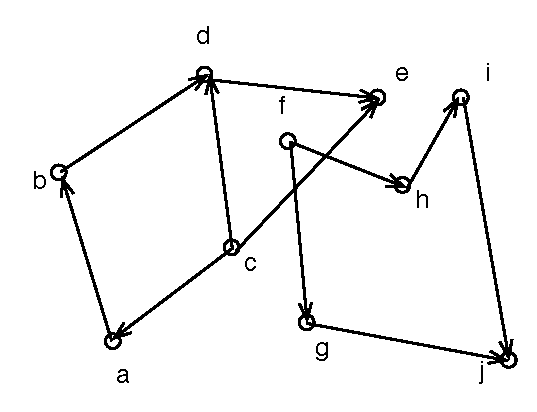
\includegraphics[width=6cm]{map.pdf}}}
%\end{figure}

%Write a Prolog database consisting of the following predicates:

%\begin{enumerate}
%\renewcommand{\theenumi}{\alph{enumi}}

%\item \texttt{line(p1,p2)} that is true iff there is a direct connection between \texttt{p1} and \texttt{p2}.

%\item \texttt{triangle(p1,p2,p3)} that is true iff \texttt{p1}, \texttt{p2}, and \texttt{p3} form a triangle (independent of the connection directions).

%\item \texttt{quadrangle(p1,p2,p3,p4)} that is true iff \texttt{p1}, \texttt{p2}, \texttt{p3}, and \texttt{p4} form a quadrangle (independent of the connection directions).

%\item \texttt{reachable(p1,p2)} that is true iff there is a directed path from \texttt{p1} to \texttt{p2} (i.e. iff \texttt{p2} is reachable from \texttt{p1} respecting the connection directions).
%\end{enumerate}

%\solution{\fontsize{8pt}{10pt}\verbatimtabinput{ex4.tex}}

% - - - - - - - - - - - - - - - - - - - - - - - - - - - - - - - - - - - - - - - - - - - - - - - - - - - - - - - - - - - - - - - - - - -



\end{document}
